% Copyright 2004 by Till Tantau <tantau@users.sourceforge.net>.
%
% In principle, this file can be redistributed and/or modified under
% the terms of the GNU Public License, version 2.
%
% However, this file is supposed to be a template to be modified
% for your own needs. For this reason, if you use this file as a
% template and not specifically distribute it as part of a another
% package/program, I grant the extra permission to freely copy and
% modify this file as you see fit and even to delete this copyright
% notice. 

\documentclass{beamer}
\setbeamertemplate{navigation symbols}{}
%\useoutertheme{shadow}
\setbeamertemplate{headline}{}

\usepackage{amssymb}
\usepackage{amsthm}
\usepackage{amstext}
\usepackage{amsbsy}
\usepackage{amscd}
\usepackage{enumerate}
\usepackage{chngpage}
\usepackage{mathtools}
\usepackage{amsmath}
\usepackage{hyperref}
\usepackage{tikz}
%\usepackage{stmaryrd}
\usepackage{color}
\usepackage{wrapfig}

\theoremstyle{plain}


\newtheorem{alg}{Algorithm}
\newtheorem{thm}{Theorem}[section]
\newtheorem{lem}[thm]{Lemma} 
\newtheorem{cor}[thm]{Corollary}
\newtheorem{prop}[thm]{Proposition}
\theoremstyle{definition}
\newtheorem{defn}[thm]{Definition}
\newtheorem{question}[thm]{Question}
\newtheorem{conj}[thm]{Conjecture}
\newtheorem{obs}[thm]{Observation}
\newtheorem{claim}[thm]{Claim}
\newtheorem{rmk}[thm]{Remark}

\newcommand{\Z}{\mathbb Z}
\newcommand{\N}{\mathbb N}
\newcommand{\R}{\mathbb R}
\newcommand{\C}{\mathbb C}
\newcommand{\Q}{\mathbb Q}
\newcommand{\F}{\mathbb F}
\newcommand{\Fp}{\mathbb{F}_p}
\newcommand{\Fq}{\mathbb{F}_q}

\newcommand{\sthat}{\,|\,}
\newcommand{\stp}[1]{\st\left(#1\right)}

\newcommand{\hal}[1]{\mathrm{hal}(#1)}
\newcommand{\gal}[1]{\mathrm{gal}(#1)}

\newcommand{\reals}{\mathbb{R}}
\newcommand{\hreals}{\prescript{*}{}{\mathbb{R}}}
\newcommand{\nats}{\mathbb{N}}
\newcommand{\hnats}{\prescript{*}{}{\mathbb{N}}}

\newcommand{\hr}[1]{\prescript{*}{}{#1}}

\newcommand{\del}{\partial}

\DeclareMathOperator{\dom}{dom}
\DeclareMathOperator{\st}{st}
\DeclareMathOperator{\inx}{inx}

\usepackage{biblatex}
\addbibresource{Thesis_Bibliography.bib}

\usepackage{graphicx}
\graphicspath{ {./images/}}
\usepackage{subcaption}



% There are many different themes available for Beamer. A comprehensive
% list with examples is given here:
% http://deic.uab.es/~iblanes/beamer_gallery/index_by_theme.html
% You can uncomment the themes below if you would like to use a different
% one:
%\usetheme{AnnArbor}
%\usetheme{Antibes}
%\usetheme{Bergen}
%\usetheme{Berkeley}
%\usetheme{Berlin}
%\usetheme{Boadilla}
\usetheme{boxes}
%\usetheme{CambridgeUS}
%\usetheme{Copenhagen}
%\usetheme{Darmstadt}
%\usetheme{default}
%\usetheme{Frankfurt}
%\usetheme{Goettingen}
%\usetheme{Hannover}
%\usetheme{Ilmenau}
%\usetheme{JuanLesPins}
%\usetheme{Luebeck}
%\usetheme{Madrid}
%\usetheme{Malmoe}
%\usetheme{Marburg}
%\usetheme{Montpellier}
%\usetheme{Metropolis}
%\usetheme{PaloAlto}
%\usetheme{Pittsburgh}
%\usetheme{Rochester}
%\usetheme{Singapore}
%\usetheme{Szeged}
%\usetheme{Warsaw}

%\usecolortheme{albatross}
%\usecolortheme{beetle}
%\usecolortheme{crane}
%\usecolortheme{dove}
%\usecolortheme{fly}
%\usecolortheme{seagull}
%\usecolortheme{wolverine}
%\usecolortheme{beaver}
%\usecolortheme{lily}
%\usecolortheme{orchid}
%\usecolortheme{rose}
%\usecolortheme{whale}
\usecolortheme{seahorse}
%\usecolortheme{dolphin}

%%%SPACING
%\let\olditem\item
%\renewcommand{\item}{\setlength{\itemsep}{\fill}\olditem}

%\useoutertheme{split}
%\setbeamertemplate{navigation symbols}{}

\makeatletter
\setbeamertemplate{footline}{}

\makeatother
\usepackage{booktabs}
\usepackage{xcolor}
\usepackage{tikz}
\usetikzlibrary{calc}

\definecolor{purple}{RGB}{155, 13, 184}
\definecolor{pink}{RGB}{252, 53, 213}
\definecolor{teal}{RGB}{4, 189, 191}

\newcommand\zp{\normalfont{\raisebox{.5pt}{\textcircled{\raisebox{-.9pt} {z}}}}}
\newcommand\rp{\normalfont{\raisebox{.5pt}{\textcircled{\raisebox{-.9pt} {r}}}}}
\newcommand\rpp{\normalfont{\raisebox{.5pt}{\textcircled{\raisebox{-.9pt} {r'}}}}}

\definecolor{myGreen}{rgb}{0.09, 0.45, 0.27}
%\usecolortheme[named=myGreen]{structure}
 
%you can put the title, author, and date here
\title{Nonstandard Analysis}

\author{Paul Schulze}

\date{}

%you always need to begin with this
\begin{document}
	
%this creates the title page
\begin{frame}
	\titlepage
\end{frame}
	
%\begin{frame} creates a slide. You put the slide title in {} directly after \begin{frame}.
	
\begin{frame}{History}
	\begin{itemize}
		\item Newton \& Leibniz formulated calculus using the idea of \textit{infinitesimals}
		\item Infinitesimals are really really small, but not $0$
		\item Considered nonsensical, replaced with $\delta$-$\epsilon$
		\item 1960s: Abraham Robinson formalizes Nonstandard Analysis
		\item Most modern formulations are based on work by Jerzy \L o\'s
	\end{itemize}
	\begin{figure}[h]
		\begin{subfigure}{0.4\textwidth}
			\centering
			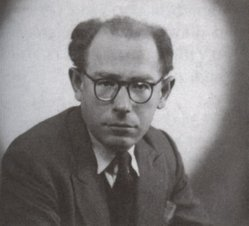
\includegraphics[width=0.6\linewidth]{Robinson}
			\caption{Abraham Robinson}
		\end{subfigure}
		\begin{subfigure}{0.4\textwidth}
			\centering
			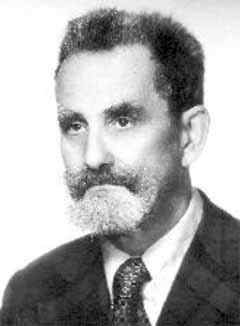
\includegraphics[width=0.4\linewidth]{Los}
			\caption{Jerzy \L o\'s}
		\end{subfigure}
	\end{figure}
\end{frame}

\begin{frame}{Hyperreals} 
We construct a set of \textit{hyperreals}, call it $\hreals$, such that we know three things: \vspace{4pt}
\begin{enumerate} \itemsep = 6pt
	\item $\reals \subseteq \hreals$
	\item $\hreals$ contains at least one infinitesimal $\delta$, such that $0 < \delta$ but $\delta < r$ for any positive real number $r$
	\item \textbf{Transfer Principle:} Any sentence of first-order logic is true in $\reals$ iff it is true* in $\hreals$
\end{enumerate}
\end{frame}

\begin{frame}{First-Order Logic}
\begin{itemize} \itemsep = 6pt
	\item Our logical language has, in addition to symbols for numbers, sets, and functions on real numbers, the following logical symbols:
	\begin{itemize}
		\item $\neg$ for ``not''
		\item $\to$ for ``if\ldots then\ldots''
		\item $\forall$ for ``for all''
		\item $\exists$ for ``there exists''
		\item $\in$ for set membership
	\end{itemize} 
	\item $5 + 3 = 8$
	\item $(\forall x \in \reals)(5 + x = 8 \to x = 3)$
	\item $(\forall x \in \reals)(\exists n \in \nats)(x < y)$
	\item $(\forall x \in \reals)(\forall n \in \nats)(x < \frac{1}{n} \to n < \frac{1}{x})$
\end{itemize}
\end{frame}

\begin{frame}{Transfer Principle}
Every sentence that's true in $\reals$ is also ``true in $\hreals$,'' when modified to be talking about $\hreals$. For instance: \vspace{6pt}
\begin{itemize} \itemsep = 8pt
	\item $(\forall x \in \hreals)(\forall y \in \hreals)(x + y = y + x)$, i.e. addition is commutative
	\begin{itemize}
		\item We can similarly prove other arithmetic properties, so we can do algebra as normal in $\hreals$
	\end{itemize}
	\item $(\forall x \in \hreals)\left(x \neq 0 \to (\exists y \in \hreals)(x \cdot y = 1)\right)$, i.e. for any nonzero $x$ there exists a multiplicative inverse $\frac{1}{x}$
	\begin{itemize}
		\item So even if $\delta$ is an infinitesimal, we know $\frac{1}{\delta}$ has to exist
	\end{itemize}
\end{itemize}
\end{frame}

\begin{frame}{What is $\hreals$ like?} 
\begin{itemize} \itemsep = 8pt
\item Call a hyperreal $x$ \textit{infinitesimal} when $|x| < r$ for every positive real $r$. 
	\begin{itemize}
	\item There's exactly one real infinitesimal: $0$
	\end{itemize}
\item There are ``infinite'' hyperreals---take any positive infinitesimal $\delta$, and $\frac{1}{\delta}$ is greater than any real number
\item Two hyperreals $x$ and $y$ are \textit{infinitely close}, denoted $x \simeq y$, when their difference $x - y$ is infinitesimal
	\begin{itemize}
	\item No two distinct real numbers are infinitely close to each other
	\item Transitive: if $x \simeq y$ and $y \simeq z$, then $x \simeq z$
	\end{itemize}
\item Any finite hyperreal $x$ is infinitely close to exactly one real number, called its \textit{standard part} $\stp{x}$
	\begin{itemize}
	\item For instance, $\stp{1 + \delta} = 1$
	\end{itemize}
\end{itemize}
\end{frame}

\begin{frame}{Derivatives, the way Leibniz intended}
\begin{itemize}
	\item Say $f: \reals \to \reals$
	\item Fix $b \in \reals$, and let $\Delta x$ be a nonzero infinitesimal. Then 
	\begin{align*}
	f'(b) = \stp{\frac{f(b + \Delta x) - f(b)}{\Delta x}}
	\end{align*}
	so that $f'(b) \simeq \frac{f(b + \Delta x) - f(b)}{\Delta x}$.
	\item \textbf{Example:} Say $f(x) = x^2$. Then we have 
	\begin{align*}
	f'(3) &\simeq \frac{(3 + \Delta x)^2 - 3^2}{\Delta x} = \frac{9 + 6 \Delta x + (\Delta x)^2 - 9}{\Delta x} \\
		&= \frac{6 \Delta x + (\Delta x)^2}{\Delta x} = 6 + \Delta x \simeq 6.
	\end{align*}
	\item So $f'(3) \simeq 6$, so their difference is infinitesimal. But they're both \textit{real numbers}, so $f'(3) = 6$.
\end{itemize}
\end{frame}

\begin{frame}{Continuity}
	We call $f(x)$ \textit{continuous} at a point $c$ if for every hyperreal $x \simeq c$, we have $f(x) \simeq f(c)$.
	\begin{theorem}
		The composition of continuous functions is continuous.
	\end{theorem}
	\begin{proof}
		Let $c$ be some real number, and let $x \simeq c$. We want to show $(f \circ g)(x) \simeq (f \circ g)(c)$, given that $g$ is continuous at $c$ and $f$ is continuous at $g(c)$. 
		
		Since $g$ is continuous at $c$, $g(x) \simeq g(c)$. Since $f$ is continuous at $g(c)$, we have $f(g(x)) \simeq f(g(c))$.
	\end{proof}
\end{frame}

\begin{frame}{Proof: Chain Rule}
Let $f,g: \reals \to \reals$ be differentiable. Let $\Delta x$ be any infinitesimal, and $\Delta g = g(x + \Delta x) - g(x)$. Since $g'(x) = \st(\Delta g / \Delta x)$ is defined, $\Delta g$ must be infinitesimal. Then
\begin{align*}
(f \circ g)'(x) &\simeq \frac{f(g(x + \Delta x)) - f(g(x))}{\Delta x}  \\
	&= \frac{f(g(x) + \Delta g) - f(g(x))}{\Delta g} \cdot \frac{\Delta g}{\Delta x} \\ 
	&\simeq f'(g(x))\cdot g'(x)
\end{align*}
So $(f \circ g)'(x) \simeq f'(g(x)) \cdot g'(x)$. But since both of these numbers are real, they must be identical. \newline

In the case where $\Delta g = 0$, we clearly have $f(g(x) + \Delta g) - f(g(x)) = 0$ and so $(f \circ g)'(x) = 0$.
\end{frame}




\end{document}